% Problem description
The left side is a lensed tapered fiber as laser source and at the right side at the working distance there is a chip formed waveguide as signal receiver.  The purpose is to find a way to gain optimized coupling efficiency through the simulations in CST MWS Environments. 


Following is a typical demonastration of fiber-to-chip coupling.
\begin{figure}
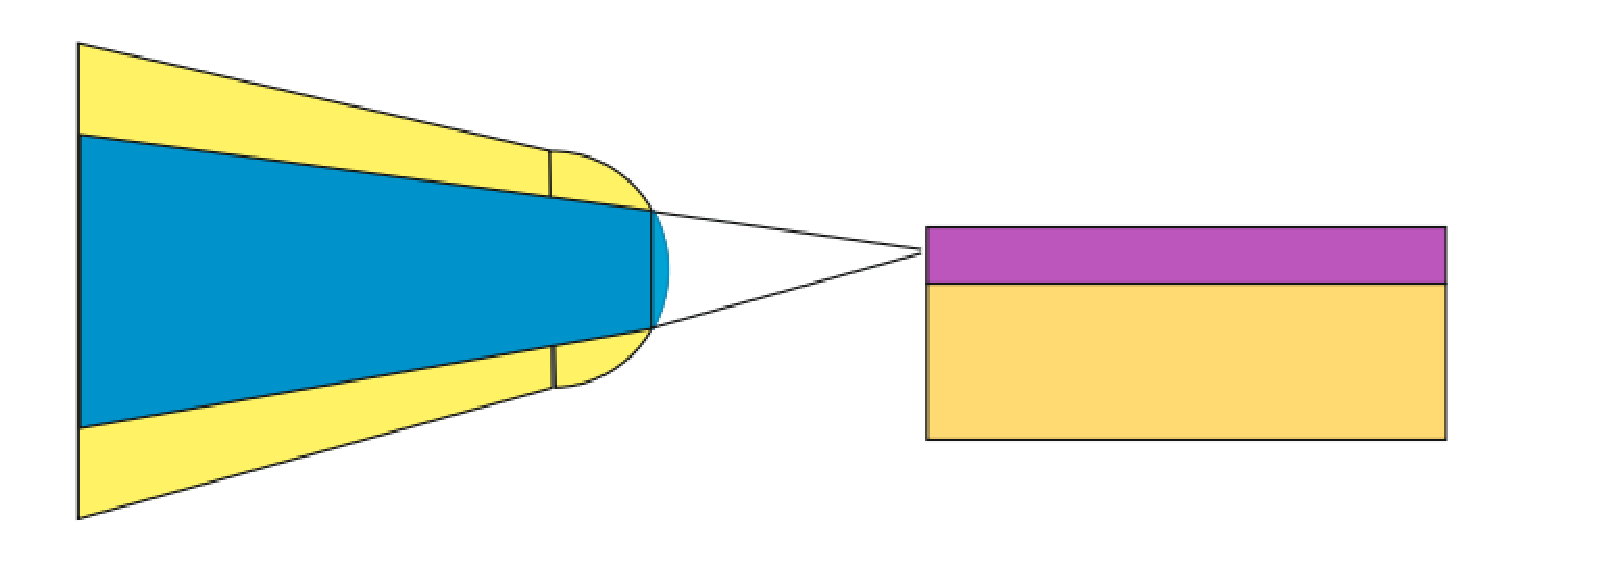
\includegraphics[width=.7\textwidth]{bilder/experiment_object}
\caption{Fiber-to-Chip Coupling}
\label{experiment_object}
\end{figure}

\begin{table}
\begin{tabular}{c|c|c}
\hline
\multicolumn{2}{|c|}{\textbf{Parameter}}&\textbf{Specification(Single-Mode)}\\
\hline
\multirow{3}{*}{Spot Size of Aspheric and Convex Lenses($1/e^2$)}&\multirow{2}{*}{Minum}&$1.7um(\lambda=1.5um)$\\
&																		 &$0.6um(\lambda=0.6um)$\\
&Maxium															 &$6.0um(\lambda=1.5um)$\\
\hline
\multirow{2}{*}{Spot Size Tolerance}&Without near-field optical characterization &$\pm 0.5um$\\
&With near-field optical characterization &$\pm 0.25um$\\
\hline
\multirow{2}{*}{Working Distance} &Minimum &$5um(\lambda=1.5um)$\\
&																	Maximum &$50um(\lambda=1.5um)$\\
\hline
	

Working Distance&
\end {tabular}
\caption{Technical parameters about tapered lensed fiber.\cite{nanoscal_tapered_fiber}}
\label{technical parameters}
\end{table}